\section{Methods}
\label{sec:methods}

This section guides through the major steps of our pipeline to get from a set of complete femur meshes and a set of partial femur meshes to a set of complete reconstructions of the partial femurs.

%% --------------------------------------------

\subsection{Setting}
\label{subsec:setting}

The implementation of our methods was done in Scala using the scalismo framework~\cite{scalismo}.
The procedure closely followed the guidelines provided by the the SICAS Medical Image Repository for their Futurelearn challenge~\cite{smir}. 
Accordingly, we used their dataset of 50 misaligned meshes of femur bones to train our model and subsequently their ten partial femur bones to test our model on.
The latter are shown in \autoref{fig:partials}.

\begin{figure*}
	\centering
  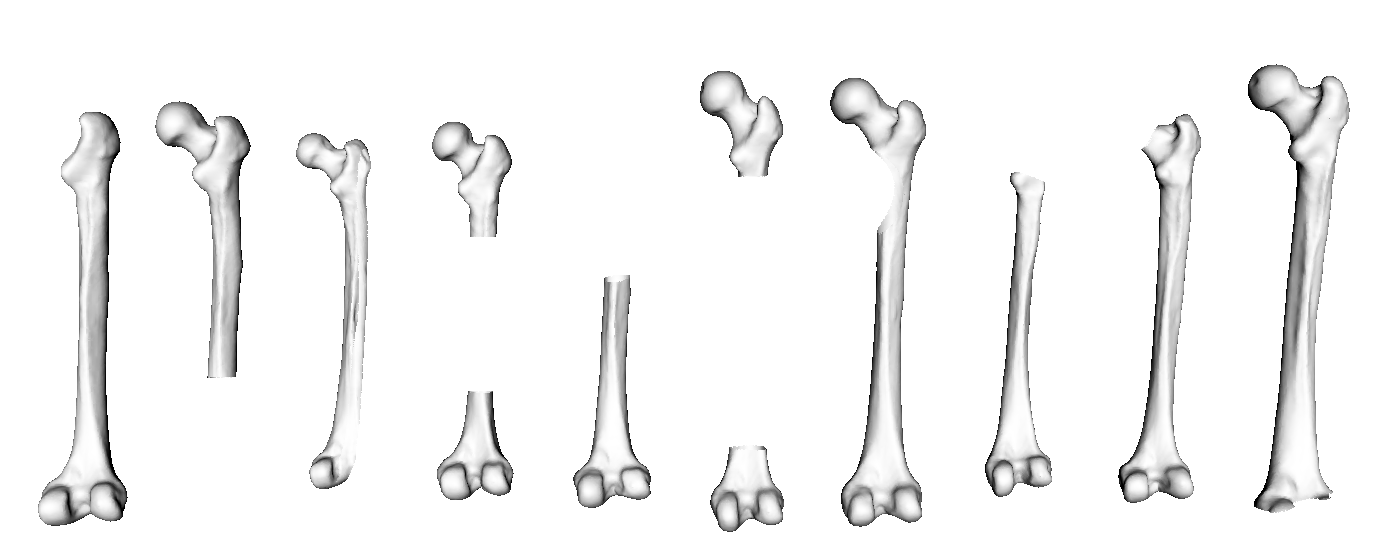
\includegraphics[width=.8\textwidth]{./Figures/partial_summary}
  \caption{The set of incomplete femur data from the SMIR competition~\cite{smir}.}
  \label{fig:partials}
\end{figure*}

%% --------------------------------------------

\subsection{Rigid Alignment}
\label{subsec:rigid}

In order for the SSM to be meaningful, we need our data to be aligned with the reference shape.
Otherwise, the main variation in the model will originate in rotation and translation of the different meshes.
Thus, in a first step, we rigidly aligned all bones given as part of the training data to the reference using a small set of landmarks also given in the data.
By minimizing the mean squared error of the corresponding landmarks, we can find a good approximation of equal orientation.
This procedure removes differences caused by translation and rotation of a shape whilst maintaining all shape information.

%% --------------------------------------------

\subsection{Shape Registration}
\label{subsec:registr}

\todoMissing{SSM from kernels (würd ich fast einen satz zu sagen -F)}
After having made sure that our femurs are oriented accordingly, our next goal was to find correspondence between them.
As their mesh representations do not necessarily have the same amount of vertices, and, furthermore, we cannot be sure that the vertices with identical identifiers are at the same place on the mesh (\eg, the tip of the femur head), we need to establish which point on one mesh corresponds to which point on the other.

The key idea here is to use a prior model and apply it to sample from the reference towards a target mesh.
As soon as the posterior is close enough to the target, we can compute its deformation to the reference for a fixed set of points on the mesh.

A simple way of approximating a target mesh is the \emph{iterative closest point algorithm} (ICP).
It non-rigidly deforms a shape according to a SSM in an iterative manner.
It searches for the points on the target mesh which are closest to a set of sample points on the deformation of the last iteration.
These points are in turn used to compute the posterior distribution.
In our implementation, we stop as soon as the change of the deformation over five iterations has fallen below a given threshold or a fixed number of iterations has been reached.

%% --------------------------------------------

\subsection{Shape Reconstruction}
\label{subsec:recon}

Given the set of deformation fields which were based on the found deformations in the previous step, we built another SSM using \emph{principal component analysis} (PCA).
On the basis of this model, we then went on estimating a sample that is as close to the parts available from our partial femur data.
For this task, we again used ICP.
Due to the fact that it is meaningless to find points closest to missing parts of the femur, however, this time we did not sample points from the mesh deformed by the algorithm, but from the partial mesh.

As the mean shape is the most probable one in a SSM, we use it as the reconstruction of the partial shape.
We have no other measure to estimate the proximity to the ground truth, as it is not provided in the data.
The evaluation from the SICAS repository is provided in Section~\ref{subsec:reconresults}.
